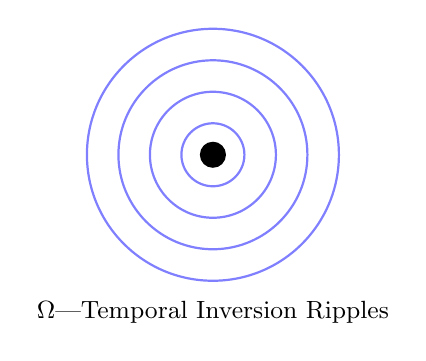
\begin{tikzpicture}[
    ripple/.style={draw=blue!50, thick},
    event/.style={circle,fill=black,minimum size=5pt}
]

\node[event] (C) at (0,0) {};

\foreach \r in {0.4,0.8,1.2,1.6}{
  \draw[ripple] (0,0) circle (\r);
}

\node at (0,-2) {\small $\Omega$---Temporal Inversion Ripples};

\end{tikzpicture}